\documentclass{article}

\usepackage{graphicx}
\usepackage{enumitem}

\begin{document}

% Nama Kelompok : Kelompok 1
% Kelas : D4 TI 1A
% 1. Dezha Aidil Martha ()
% 2. M.Tomy Maulidy ()
% 3. Habib Abdul Rasyid (1174002)
% 4. Nico Eklessia Sembiring (1174096)
% 5. Damara Benedikta Siolemba ()
% 6. Felix Setiawan Lase ()

\section{Pengertian Sensor Suhu}

\begin{figure}[ht]
	\centerline{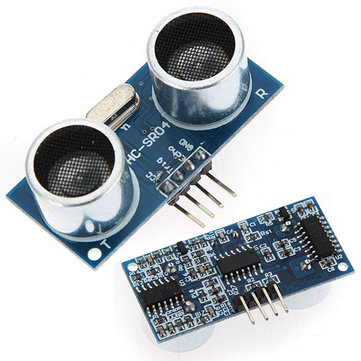
\includegraphics[width=0.4\textwidth]{figures/sensor.jpg}}
	\caption{DHT11}
	\label{DHT11}
\end{figure}

Sensor suhu dan kelembaban DHT11 merupakan sensor untuk mensensing objek suhu dan kelembaban pada 1 module yang dimana memiliki output sinyal digital yang sudah terkalibrasi.
Module sensor ini tergolong kedalam elemen resistif seperti perangkat pengukur suhu seperti contohnya yaitu NTC.
Keunggulan dari sensor DHT11 dibanding dengan yang lainnya antara lain memiliki kualitas pembacaan data sensing yang sangat baik, responsif (cepat dalam pembacaan kondisi ruangan), serta tidak mudah terinterverensi.
Pada setiap sensor DHT11 ini memiliki fitur untuk kalibrasi dari kelembaban ruang kalibrasi, dan itu kalibrasinya cukup akurat.

\section{Spesifikasi dari Modul Sensor Suhu}

Di pasaran terdapat dua macam tipe DHT11 yang umumnya sudah berupa modul, yakni DHT11 dengan 3 pin dan 4 pin. Intinya sama saja, karena pada modul DHT11 yang berkaki 4 ada satu pin yang tidak digunakan.

\begin{figure}[ht]
	\centerline{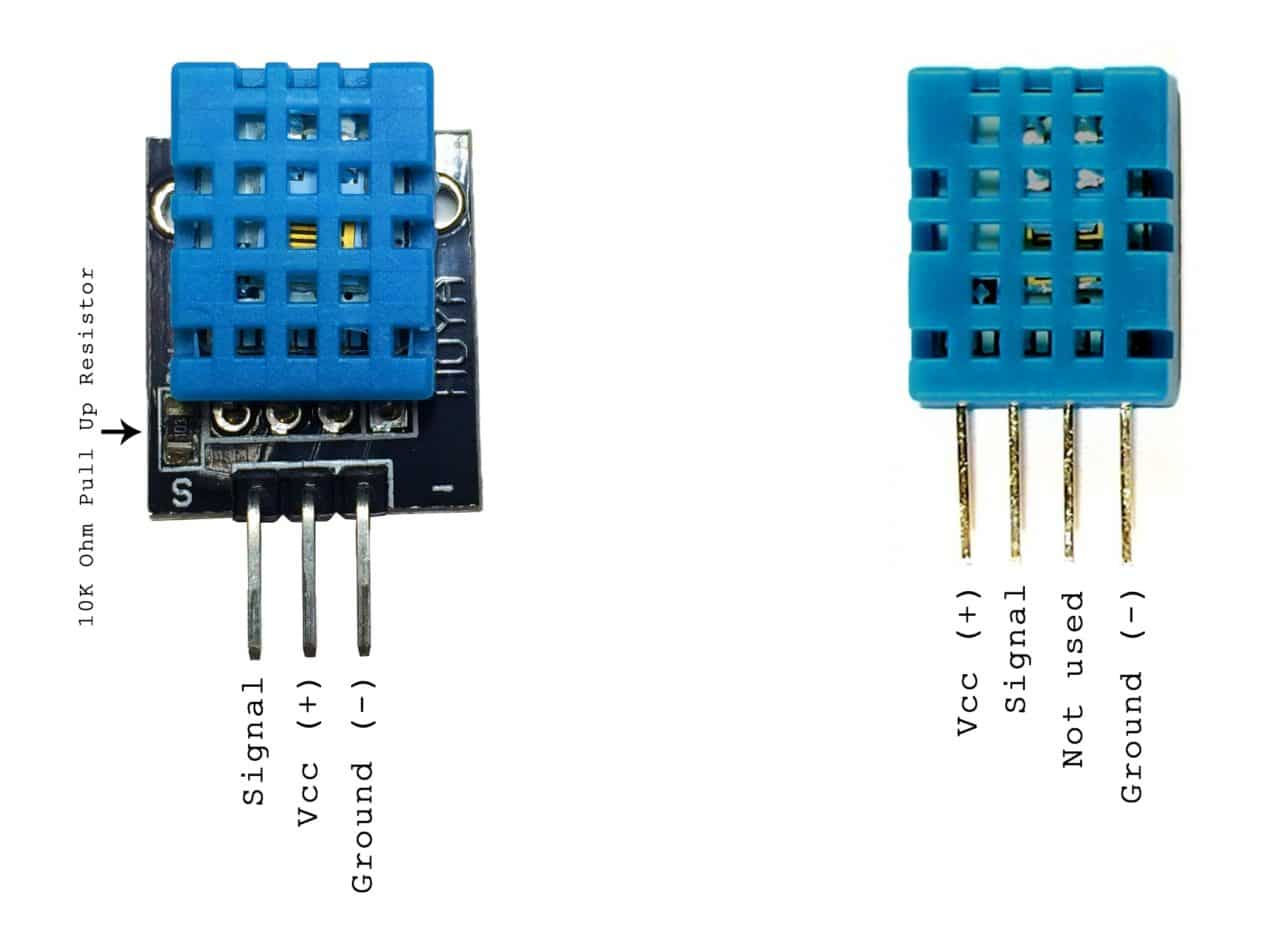
\includegraphics[width=0.4\textwidth]{figures/DHT11.jpg}}
	\caption{Sensor suhu}
	\label{DHT11}
\end{figure}

Spesifikasi dari modul sensor suara seperti contoh pada gambar adalah sebagai berikut :

\begin{itemize}
	\item Pasokan Voltage 5V.
	\item Rentan Temperatur 0-50 derajat.
	\item Kelembaban 20-90 RH.
	\item Interface Digital.
\end{itemize}

\section{Tutorial Mengakses Sensor Suhu}

\hspace{4mm} Bahan-bahan yang diperlukan untuk mengakses sensor suhu, yaitu :

\begin{itemize}
	\item Arduino Uno 
	\item Komputer + Software IDE Arduino
	\item Sensor DHT11
	\item Kabel Jumper
	\item Lampu LED
	\item Kabel USB
\end{itemize}

\break Proses pembuatan :

\begin{enumerate}
	
	\item  Pertama, pasang kabel jumper bagian female ke masing-masing pin modul sensor suhu. Kabel jumper berwarna hijau ke pin Analog Output (AO). Kabel jumper berwarna kuning ke pin Ground (G). Kabel jumper berwarna orange ke pin Voltage Common Collector (VCC).
	\break
	\centerline{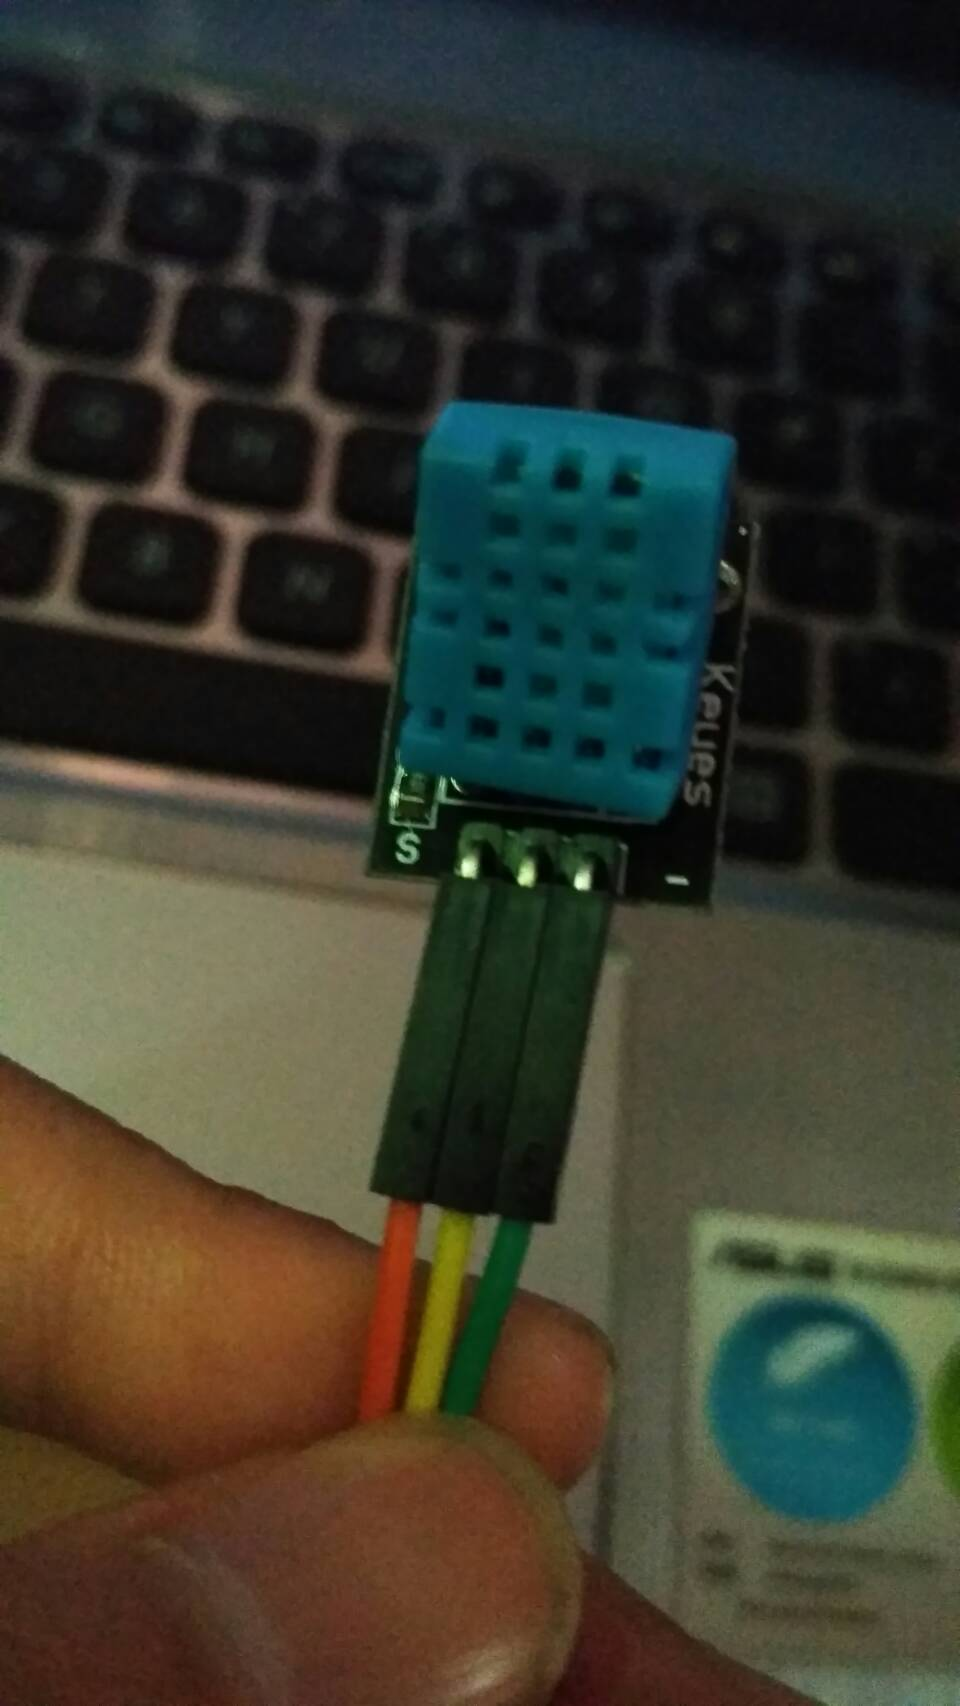
\includegraphics[width=0.9\textwidth]{figures/female.jpg}}
	\break
	\item Setelah semuanya terpasang, lalu sambungkan kabel jumper bagian male ke arduino. Kabel jumper berwarna hijau ke slot A1. Kabel jumper berwarna kuning ke slot GND. Kabel jumper berwarna orange ke slot 5V.
	\break
	\centerline{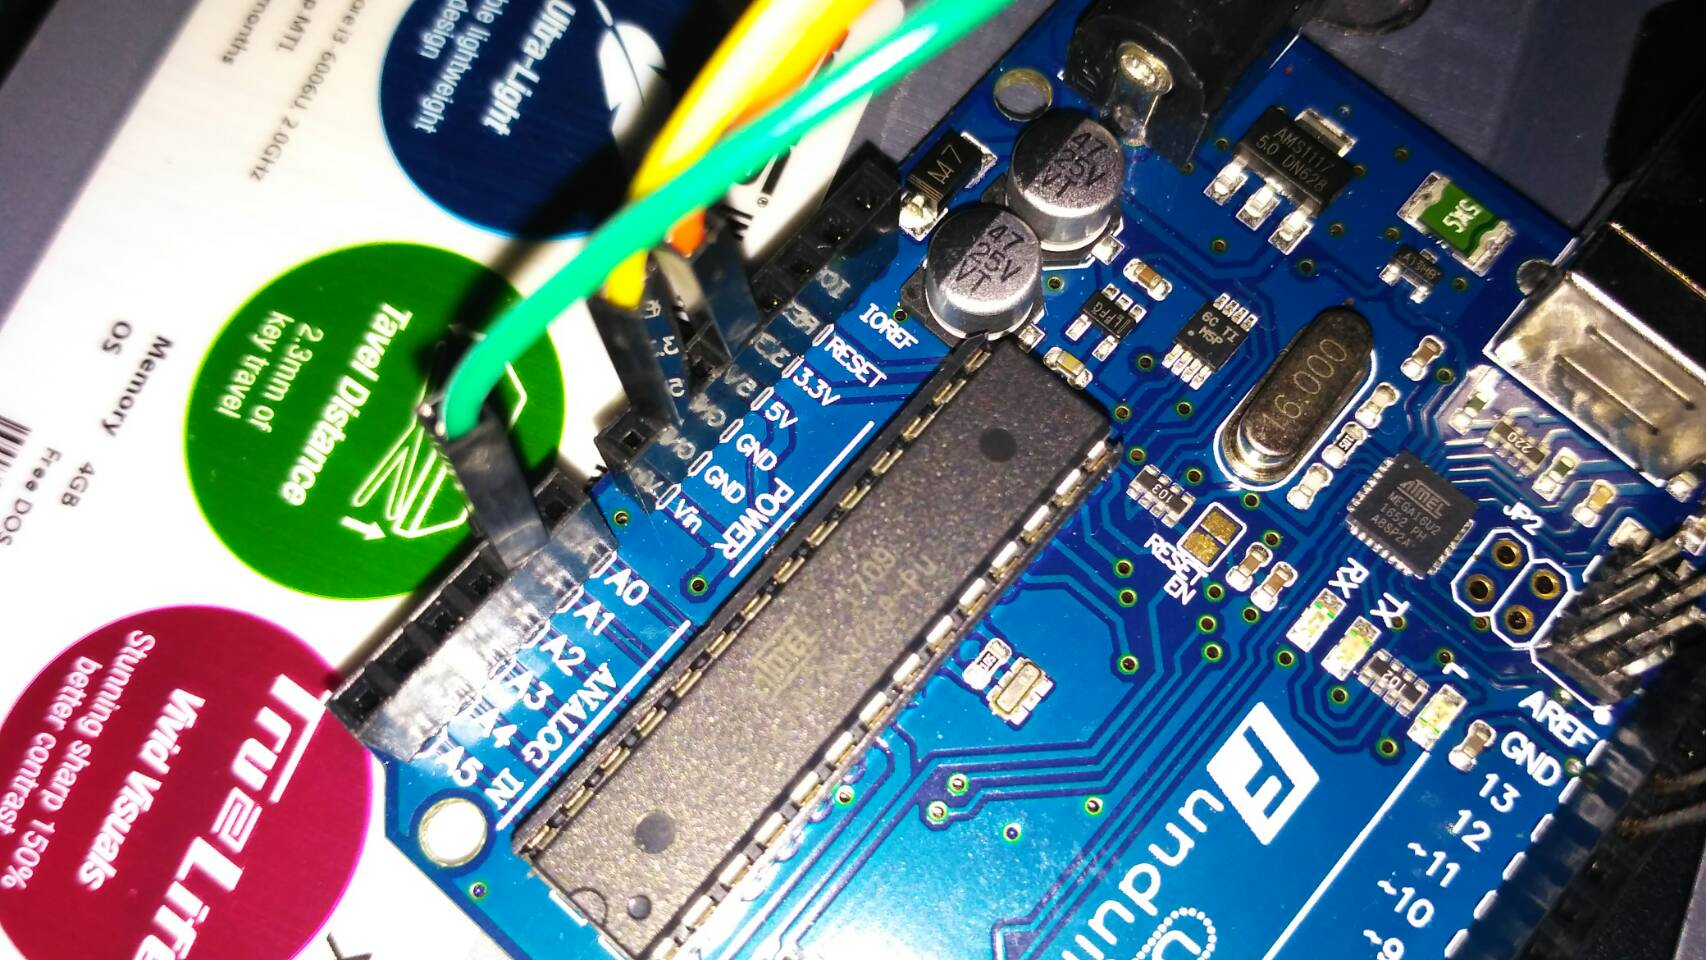
\includegraphics[width=0.9\textwidth]{figures/male.jpg}}
	\break
	\item Setelah semua terhubung, lalu sambungkan kabel USB ke arduino dan ke komputer.
	\break
	\centerline{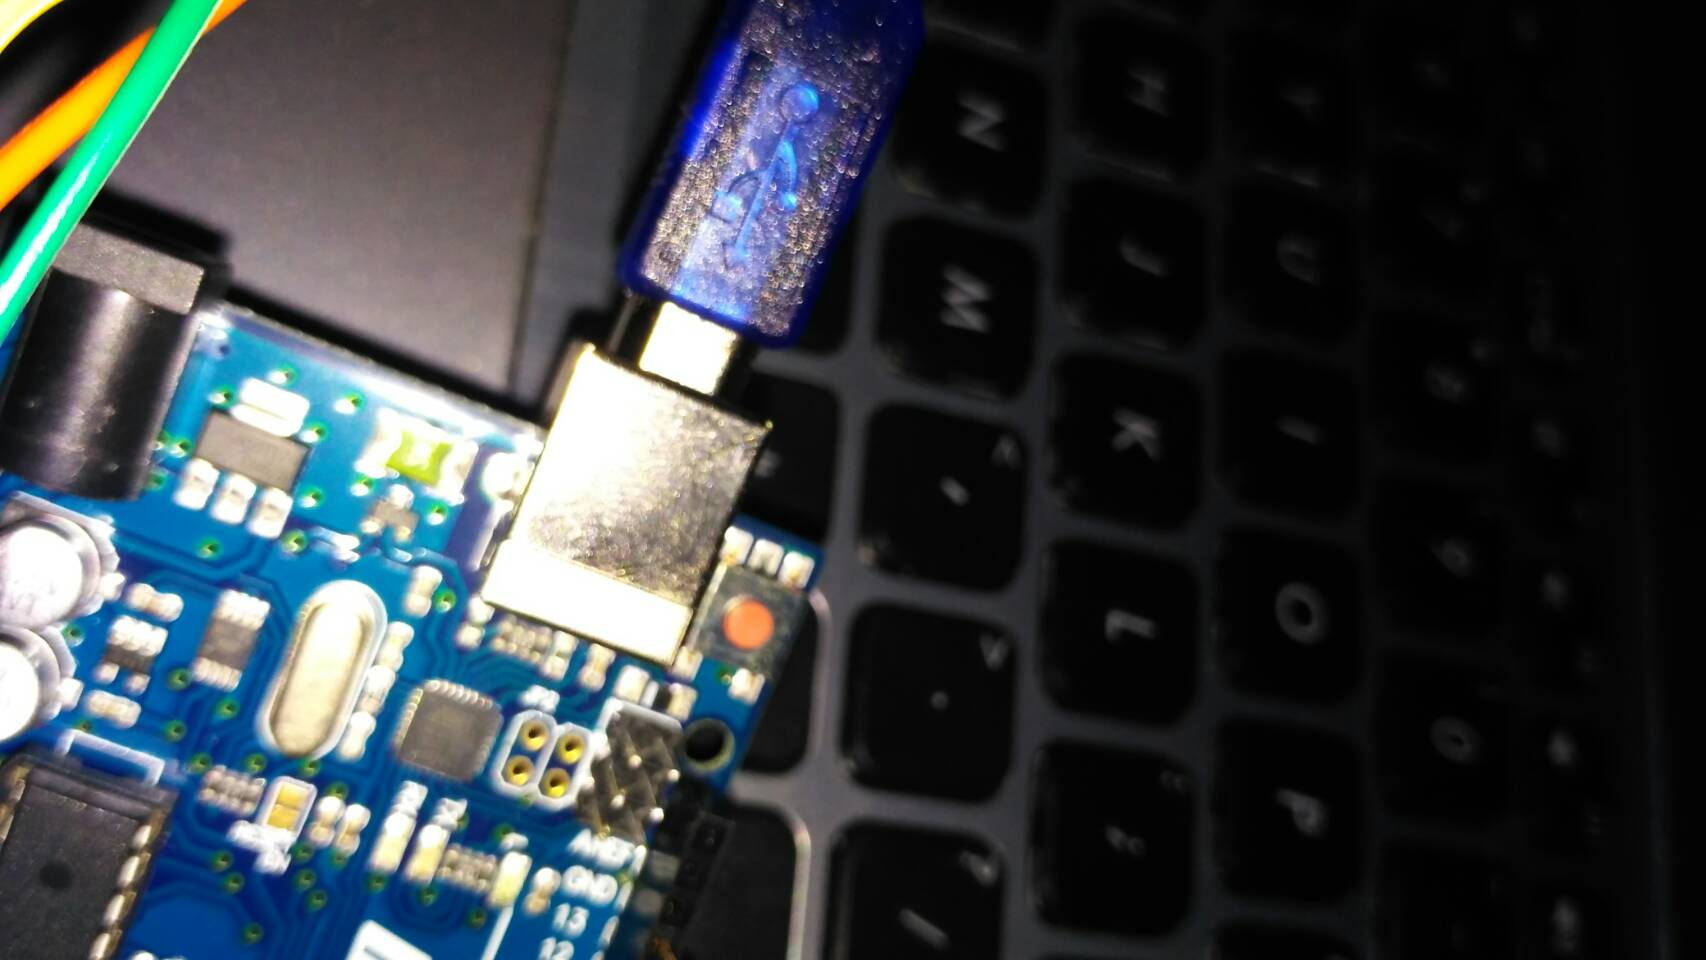
\includegraphics[width=0.9\textwidth]{figures/usb.jpg}}
	\break
	\item Lalu pasang lampu LED ke arduino. Pin yang lebih panjang pasang ke slot 13, sedangkan pin yang pendek pasang ke slot GND.
	\break
	\centerline{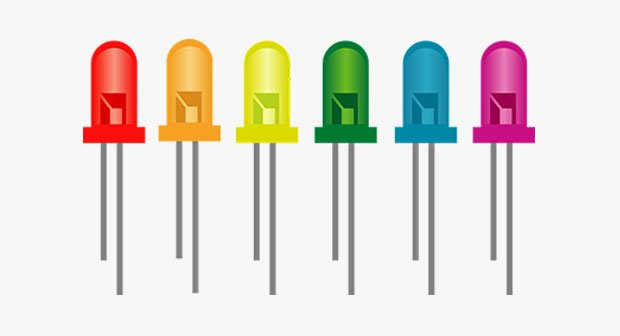
\includegraphics[width=0.9\textwidth]{figures/led.jpg}}
	\item  Kemudian buat program yang nantinya digunakan untuk mengetes sensor menggunakan IDE Arduino.
	\break
	\centerline{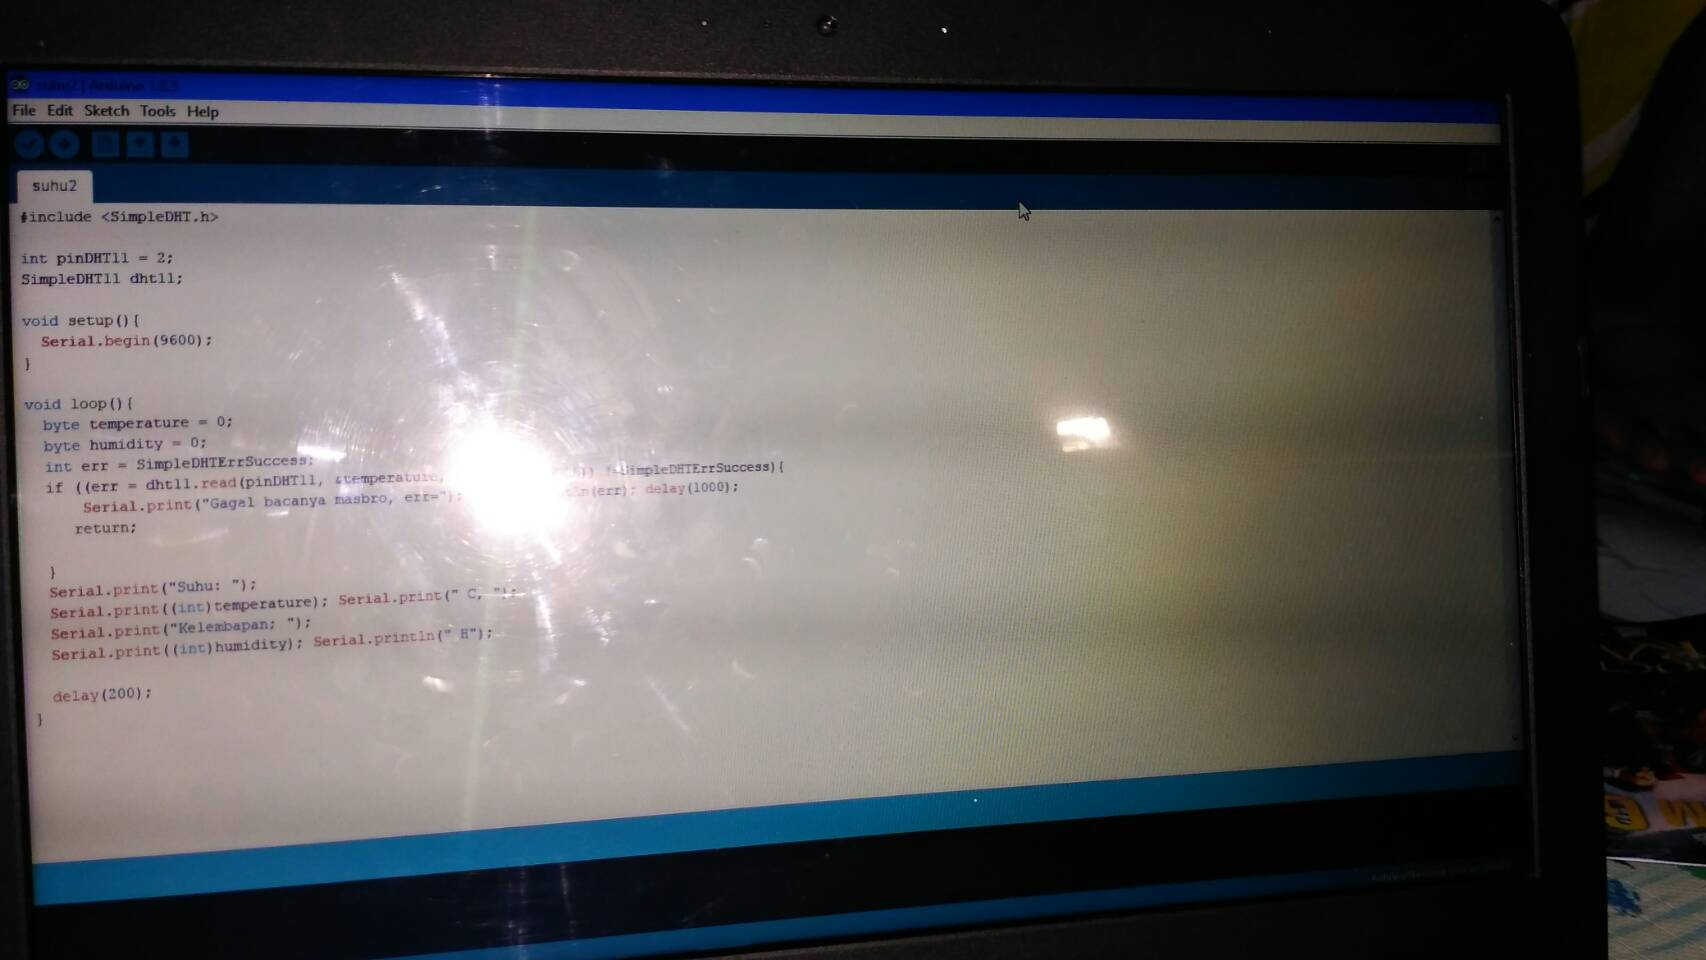
\includegraphics[width=0.9\textwidth]{figures/kode.jpg}}
	\item Lalu setelah program selesai dibuat, upload program tersebut ke arduino.
	\break
	\item Terakhir cek apakah sensor berkerja dengan semestinya.
	\break
	
\end{enumerate}

\end{document}